% -----------------------------------------------
% Template for SMC 2020
% adapted from previous SMC paper templates
% -----------------------------------------------

\documentclass{article}
\usepackage{smc2020}
\usepackage{times}
\usepackage{ifpdf}
\usepackage[italian,english]{babel}
\usepackage{cite}

%%%%%%%%%%%%%%%%%%%%%%%% Some useful packages %%%%%%%%%%%%%%%%%%%%%%%%%%%%%%%
%%%%%%%%%%%%%%%%%%%%%%%% See related documentation %%%%%%%%%%%%%%%%%%%%%%%%%%
%\usepackage{amsmath} % popular packages from Am. Math. Soc. Please use the
%\usepackage{amssymb} % related math environments (split, subequation, cases,
%\usepackage{amsfonts}% multline, etc.)
%\usepackage{bm}      % Bold Math package, defines the command \bf{}
%\usepackage{paralist}% extended list environments
%%subfig.sty is the modern replacement for subfigure.sty. However, subfig.sty
%%requires and automatically loads caption.sty which overrides class handling
%%of captions. To prevent this problem, preload caption.sty with caption=false
%\usepackage[caption=false]{caption}
%\usepackage[font=footnotesize]{subfig}


%user defined variables
\def\papertitle{SEAM PROJECT - SUSTAINED STEREOPHONY}
\def\firstauthor{Giuseppe Silvi}
\def\secondauthor{Davide Tedesco}
\def\thirdauthor{Third author}

% adds the automatic
% Saves a lot of output space in PDF... after conversion with the distiller
% Delete if you cannot get PS fonts working on your system.

% pdf-tex settings: detect automatically if run by latex or pdflatex
\newif\ifpdf
\ifx\pdfoutput\relax
\else
   \ifcase\pdfoutput
      \pdffalse
   \else
      \pdftrue
\fi

\ifpdf % compiling with pdflatex
  \usepackage[pdftex,
    pdftitle={\papertitle},
    pdfauthor={\firstauthor, \secondauthor, \thirdauthor},
    bookmarksnumbered, % use section numbers with bookmarks
    pdfstartview=XYZ % start with zoom=100% instead of full screen;
                     % especially useful if working with a big screen :-)
   ]{hyperref}
  %\pdfcompresslevel=9

  \usepackage[pdftex]{graphicx}
  % declare the path(s) where your graphic files are and their extensions so
  %you won't have to specify these with every instance of \includegraphics
  \graphicspath{{img/}}
  \DeclareGraphicsExtensions{.pdf,.jpeg,.png}

  \usepackage[figure,table]{hypcap}

\else % compiling with latex
  \usepackage[dvips,
    bookmarksnumbered, % use section numbers with bookmarks
    pdfstartview=XYZ % start with zoom=100% instead of full screen
  ]{hyperref}  % hyperrefs are active in the pdf file after conversion

  \usepackage[dvips]{epsfig,graphicx}
  % declare the path(s) where your graphic files are and their extensions so
  %you won't have to specify these with every instance of \includegraphics
  \graphicspath{{./figures/}}
  \DeclareGraphicsExtensions{.eps}

  \usepackage[figure,table]{hypcap}
\fi

%setup the hyperref package - make the links black without a surrounding frame
\hypersetup{
    colorlinks,%
    citecolor=black,%
    filecolor=black,%
    linkcolor=black,%
    urlcolor=black
}

\usepackage{color}
\usepackage{listings}
\definecolor{mygrey}{rgb}{0.96,0.96,0.96}
% lstlistings setup
\definecolor{yobg}{rgb}{0.9,0.9,1}
\definecolor{yotxt}{rgb}{0.01,0.01,0.52} % a dark blue.
\definecolor{mylstbg}{rgb}{0.98,0.98,0.98} % a really pale grey.
\definecolor{mylstcmt}{rgb}{0.01,0.52,0.01} % a dark green.
\definecolor{mylstdoc}{rgb}{0.80,0.30,0.80} % a medium pink.

\lstset{%
  language=C++,
  numbers=left,%none,
  tabsize=4,
  frame=single,
  breaklines=true,
  numberstyle=\tiny\ttfamily,
  backgroundcolor=\color{mylstbg},
  basicstyle=\scriptsize\ttfamily,
  commentstyle=\slshape\color{mylstcmt}, %\itshape,
  %frameround=tttt,
  columns=flexible, %fixed,
  showstringspaces=false,
  emptylines=2,
  inputencoding=utf8,
  extendedchars=true,
  literate=	{á}{{\'a}}1
			{à}{{\`a}}1
			{ä}{{\"a}}1
			{â}{{\^a}}1
			{é}{{\'e}}1
			{è}{{\`e}}1
			{ë}{{\"e}}1
			{ê}{{\^e}}1
			{ï}{{\"i}}1
			{î}{{\^i}}1
			{ö}{{\"o}}1
			{ô}{{\^o}}1
			{è}{{\`e}}1
			{ù}{{\`u}}1
			{û}{{\^u}}1
			{ç}{{\c{c}}}1
			{Ç}{{\c{C}}}1,
  emph={component, declare, environment, import, library, process, with},
  emph={[2]ffunction, fconstant, fvariable},
  emph={[3]button, checkbox, vslider, hslider, nentry, vgroup, hgroup, tgroup, vbargraph, hbargraph, attach},
  emphstyle=\color{yotxt}, %\underline, %\bfseries,
  morecomment=[s][\color{mylstdoc}]{<mdoc>}{</mdoc>},
  rulecolor=\color{black}
}



% Title.
% ------
\title{\papertitle}

% Authors
% Please note that submissions are NOT anonymous, therefore
% authors' names have to be VISIBLE in your manuscript.
%
% Single address
% To use with only one author or several with the same address
% ---------------
%\oneauthor
%   {\firstauthor} {Affiliation1 \\ %
%     {\tt \href{mailto:author1@smcnetwork.org}{author1@smcnetwork.org}}}

%Two addresses
%--------------
 \twoauthors
   {\firstauthor} {Affiliation1 \\ %
     {\tt \href{mailto:author1@smcnetwork.org}{author1@smcnetwork.org}}}
   {\secondauthor} {Affiliation2 \\ %
     {\tt \href{mailto:author2@smcnetwork.org}{author2@smcnetwork.org}}}

% Three addresses
% --------------
% \threeauthors
%   {\firstauthor} {Affiliation1 \\ %
%     {\tt \href{mailto:author1@smcnetwork.org}{author1@smcnetwork.org}}}
%   {\secondauthor} {Affiliation2 \\ %
%     {\tt \href{mailto:author2@smcnetwork.org}{author2@smcnetwork.org}}}
%   {\thirdauthor} { Affiliation3 \\ %
%     {\tt \href{mailto:author3@smcnetwork.org}{author3@smcnetwork.org}}}


%%%%%%%%%%%%%%%%%%%%%%%%%%%%%%%%%%%%%%%%%%%%%%%%%%%%%%% THE DOCUMENT STARTS HERE
\begin{document}
%
\capstartfalse
\maketitle
\capstarttrue
%
\begin{abstract}
\input{abstract.txt}
\end{abstract}
%

%%%%%%%%%%%%%%%%%%%%%%%%%%%%%%%%%%%%%%%%%%%%%%%%%%%%%%%%%%%%%%%%%%%% SECTION ONE
%%%%%%%%%%%%%%%%%%%%%%%%%%%%%%%%%%%%%%%%%%%%%%%%%%%%%%%%%%%%%%%%%%%%%%%%%%%%%%%%
\section{Introduction}
\label{sec:introduction}

\emph{Sustained Electro-Acoustic Music} is a project inspired by Alvise Vidolin
and Nicola Bernardini's article \cite{bevi05} on \emph{live electroacoustic
music sustainability}.

The main ambition of this project is to grow the interpretation and the
electroacoustic musical practice with the consciousness of the electronic
and informatics problems that had made arduous to approach this music and
prevented the growth of interpretative thinking. It is possible, with a
community structure, to determine, build and stratify interpretation of musical
core, the repertoire, concealing the environment-related technological issues.
They are instruments, not the music itself, after all.

These are the SEAM organisation coordinates:
\begin{itemize}
\item \url{http://s-e-a-m.github.io}
\item \url{http://seam-world.slack.com}
\end{itemize}

\vfill\null

\newpage

%%%%%%%%%%%%%%%%%%%%%%%%%%%%%%%%%%%%%%%%%%%%%%%%%%%%%%%%%%%%%%%%%%%% SECTION TWO
%%%%%%%%%%%%%%%%%%%%%%%%%%%%%%%%%%%%%%%%%%%%%%%%%%%%%%%%%%%%%%%%%%%%%%%%%%%%%%%%
\section{PROBLEMS}
\label{sec:problems}

Why a project about sustained electroacoustic music must focus on stereophony issues? The literature and the repertoire survive thanks to the community activities. Most of those activities require education, strong education about sound and musical matters, layered, from roots to top floor of knowledge.

Especially the roots, the elementary concepts, the etymology of the basic lexis, is the most fragile and most violated place of knowledge, a place where stereophony, one of the keywords of the sound realm, just before to lose its meaning still losing its necessity.

Speaking about stereophonic sound in music classes, at each level of learning, should be a keynote, a moment in which by simple words, simple by different level of learning, people can understand how they listen to something, perhaps the music, they also understand the sound reproduction meaning, with reproduction significance of something real, where per real we focus at least on what we perceive and able to describe, like about sound. So, in music, speaking of listening and, after, stereophony, must be a grade zero of comprehension and, after, knowledge. How it could happen if the explanations about sounds, reproduction of sounds and stereophonic sounds are the following?

\begin{quotation}
È bene chiarire subito la differenza fra il concetto di “mono” e quello di “stereo”. Mono è un termine che deriva dal greco e vuol dire «solo», «formato da uno solo». Nel campo audio si definisce mono un segnale che viaggia su un solo canale; esso è costituito da un'unica onda. Si definisce Stereo una coppia di segnali audio aventi delle differenze anche minime fra loro, che viaggia su due canali indipendenti: il canale sinistro e il canale destro; il segnale stereo è pertanto costituito da due onde\footnote{It is good to immediately clarify the difference between the concept of "mono" and that of "stereo". Mono is a term that derives from the Greek and means "solo", "made up of just one". In the audio field, a signal that travels on a single channel is defined as mono; it consists of connected wave. Stereo is defined as a pair of audio signals having even minimal differences between them, which travels on two independent channels: the left channel and the right channel; the stereo signal consists of two waves. (The Book here cited is the most adopted by Italian Musical High School)}. \cite{labtec01}
\end{quotation}

\ldots and many greetings to Blumlein.

Which electroacoustic realm could be based on these explanations? The one we internationally have now. The one that totally ignores the loss of the necessity of listening with both ears. The most music, audible during electroacoustic concerts and live interactive performances, in particular the one made with high technology sensors and interactive features, easily does not focus at all on how people will listen to the performance. At the question “which is your music staging plan?” the most diffused worst answer is “stereo”. Worst, because it is untrue, because they do not know what are saying and doing.

The first consequence of missing two-ears-attitude in the electroacoustic domain is the persistence of works that not have the necessity of audience, of auditorium neither. We do not even know who is the chicken or the egg, we only can underline the bond of them.

Nevertheless, the authors \cite{labtec01} of the text above cited, in the preface they claim the necessity of a didactic book, a text to take on during the early stage of music technology learning. They are full of interpretations to allow oneself to follow the unstoppable urge of writing books for young students, instead give them The Gift, the best instruction to be passed to people who caress the roots: how to search the meaning of things on literature and, especially, the encyclopedia\footnote{
The Italian Treccani encyclopedia at \\
\url{http://www.treccani.it/enciclopedia/stereofonia/} \\
explain with universally-simple words what humanity, without allowing to personal interpretations, should refer with stereophony words. It is free knowledge, for Italian speaking people, not overwritten-able. We ironically even must sustain the use of the encyclopedia.}.

So, to argue our point, why focus on greek etymology of \emph{mono}, \emph{alone}, and not of \emph{stereo}, from greek \emph{Stereos}, \emph{solid}. Maybe because it means not a number, not a configuration, only an adjective. Again, \emph{solid}, \emph{firm and stable in shape}, \emph{having three dimensions}. \emph{Solid}, from Latin root of \emph{Solidus}, \emph{Sollus}, \emph{entire}.

We also prefer to underline that \emph{mono} is the nickname for \emph{monophonic}, with the bond between \emph{monos} and \emph{phon\={e}}, \emph{one voice}, \emph{alone}. The same word used in a Gregorian chant description, later evolved in polyphony (from Greek \emph{poluph\={o}nia}, from \emph{polu}, \emph{many} and \emph{phon\={e}}). So the dichotomy, if must be one, between monophony and stereophony simply does not exist. The extension of monophony concept is the polyphony. Stereophony is simply another concept.

With the word Stereophony, we should describe a condition by which a \emph{Phon\={e}}, voice, sound, arrival solid to the listener, whole, firm and stable in their multidimensional sound shape, even in its electroacoustic reproduction, with any necessary number of channels.

The path of this journey in the middle-earth of stereophony wants to lead to an understanding of the complexity and unsolved issues around electroacoustic sound reproduction. It is not a text on a new approach to something, rather it is an old something to be re-assembled, to be re-read, a path to seam and bond of different ideas appeared in our history of music, to which we, musicians, must be referred when staging music. The journey will not complete itself. The path will not lead somewhere. The real sustaining of electroacoustic music will start only with the death of the ready-to-listen recipes approach. When listening and speculation on music and sound will come back fashionable. 

\vfill\null

\newpage

%%%%%%%%%%%%%%%%%%%%%%%%%%%%%%%%%%%%%%%%%%%%%%%%%%%%%%%%%%%%%%%%%% SECTION THREE
%%%%%%%%%%%%%%%%%%%%%%%%%%%%%%%%%%%%%%%%%%%%%%%%%%%%%%%%%%%%%%%%%%%%%%%%%%%%%%%%
\section{ROOTS}
\label{sec:roots}

The healthy mental attitude to sharing knowledge forecast the roots knowledge and sharing, even without interpretations, they could be afforded later.

\begin{quotation}
An observer in the room is listening with two ears, so that echoes reach him
with the directional significance which he associates with the music performed
in such room. He therefore discount these echoes and psychologically focuses
his attention on the source of the sound. When the music is reproduced through
a single channel the echoes arrive from the same direction as the direct sound
so that confusion results. [\ldots] Human ability to determine the direction from which sound arrives is due to binaural hearing, the brain being able to detect differences between sound received by the two ears from the same source and thus to determine angular directions from which various sounds arrive. \cite{ab58}
\end{quotation}

With those words, Blumlein \cite{ab58} described simultaneously the fundamentals of at least two huge arguments: how we perceive acoustic sounds, how we had reproduced sounds until that moment to be listened to and perceived.

Is a single human voice speaking, a monophonic voice inside a small room, an acceptable stereophonic condition? In agreement with Blumlein, Yes! This is the first firm point.

The binaural-ity of the human listening as the first statement of Blumlein conception: “\emph{an observer in the room is listening with two ears}”.

Michael Gerzon, from the roots of Blumlein and friends, jump the line with a clear description 

\begin{quotation}
The ears and brain localize sounds according to many different mechanism. Among the most important cues used are low frequency interaural phase (applicable up to around 2\emph{KHz}, but dominant below 700\emph{Hz}) and localization by amplitude differences between the two ears, predominantly above about 1\emph{KHz}. While other cues are also important, we have found that satisfying both these cues, and making them mutually consistent for central listener facing inn any direction, leads to particularly robust and reliable localization quality.\cite{mg92pdmsss}
\end{quotation}

\vfill\null

\newpage

%%%%%%%%%%%%%%%%%%%%%%%%%%%%%%%%%%%%%%%%%%%%%%%%%%%%%%%%%%%%%%%%%%% SECTION FOUR
%%%%%%%%%%%%%%%%%%%%%%%%%%%%%%%%%%%%%%%%%%%%%%%%%%%%%%%%%%%%%%%%%%%%%%%%%%%%%%%%
\section{Branches}
\label{sec:branches}

With the deep knowledge of time meaning between us and Blumlein, we can expose loudspeaker significance better than him. For the Blumlein era, the loudspeaker was the future instrument for a better present time. The reproduced sound, at its young age, was pure magic. Today we know well how unsatisfied we are of loudspeaker reproduction. When the first iPhone was the only one smart-thing on the planet, it was awesome an awesome object of crafting. Today with the same object we would not take even a picture. Listening to a violin solo reproduced by the best loudspeaker on the market is not the same experience of the real performance. It is not related to stereophony and technique ability, it is integral to the reproduction limit of the technology we are able to craft.

Replacing the human voice speaking with a loudspeaker speaking the just now recorded human voice we lose, as Blumlein described, the capacity of ears-brain deciphers the sound-environment relationship. It is not more a stereophonic listening.

\begin{quotation}
we show the loudspeaker layouts considered fo frontal stage stereo using from one (regarding mono as the trivial case of “one-loudspeaker stereo”!) to five loudspeakers… \cite{mg92pdmsss}
\end{quotation}

\vfill\null

\newpage

%%%%%%%%%%%%%%%%%%%%%%%%%%%%%%%%%%%%%%%%%%%%%%%%%%%%%%%%%%%%%%%%%%% SECTION FIVE
%%%%%%%%%%%%%%%%%%%%%%%%%%%%%%%%%%%%%%%%%%%%%%%%%%%%%%%%%%%%%%%%%%%%%%%%%%%%%%%%
\section{Mid-Side}
\label{sec:midside}

\begin{lstlisting}
nsum = 0.5*(_+_);
ndif = 0.5*(_-_);
sdmx = _,_ <: nsum, ndif;
\label{ls:sdmx}
\end{lstlisting}

\begin{quotation}
…it is fairly well established that the main factor having effect are phase
differences and intensity differences between the sounds reaching the two ears,
the influence with each of these has depending upon the frequency of the sounds
emitted. For low frequency sound waves there is little or non difference in
intensity at the two ears but there is a marked phase difference. For a give
obliquity of sound the phase difference is approximately proportional to
frequency, representing a fixed time delay between sound arriving at the two
ears, by noting which there is a phase difference of pi radians or more between
sound arriving at the two ears from a source located on the line joining them:
but above such frequency if phase difference were the sole feature relied upon
for directional location there would be ambiguity in the apparent position of
the source. At the stage however the head begins to became effective as a baffle
and causes noticeable intensity difference between the sounds reaching the two
ears, and it is by noting such intensity difference that brain determines
direction of sounds at higher frequencies.
\end{quotation}

\begin{quotation}
…the frequency at which the brain changes over from phase- to
intensity-discrimination occurs at about 700cps. …inn any case the transference
is not sudden or discontinuous but there is considerable overlap of the two
phenomena so that over a considerable frequency range differences of both phase
and intensity will to some extent have an effect ion determine the sense of
direction experienced.
\end{quotation}

\begin{quotation}
The invention also consists in a system of sound transmission wherein the sound
is receive by two or more microphones, wherein at low frequencies difference in
the phase of sound pressure at the microphone is reproduced as difference in
volume at the loud speaker.
\end{quotation}

\vfill\null

\newpage

%%%%%%%%%%%%%%%%%%%%%%%%%%%%%%%%%%%%%%%%%%%%%%%%%%%%%%%%%%%%%%%%%%%% SECTION SIX
%%%%%%%%%%%%%%%%%%%%%%%%%%%%%%%%%%%%%%%%%%%%%%%%%%%%%%%%%%%%%%%%%%%%%%%%%%%%%%%%
\section{Mid-Side Panner}
\label{sec:mspanner}

During the lessons in Rome Conservatory in which \emph{SEAM} was born and its
related problems were shared with classes to sensitize students to community
work, the core software used to explode issues was \emph{Faust}\footnote{
\url{https://faust.grame.fr}}. This wasn't a restriction, it was a preference.
Text-based DSP offers the deepest learning experience and great expressivity
and readability. \emph{Faust} code could be written to educate a musician at
the same time with computation versatility and efficiency. The \emph{Faust
libraries} concept is useful to focus on write once, and read forever, code.
We think \emph{Faust} itself represents a rather concept of electroacoustic
sustainability. Thinking, for example, at the \emph{filters.lib} and at the
names that contributed the enrichment of speculation around each object, make
us wish to a musical interest capable to do community more than with the
adoption of other software.

Instruments carved by musical ideas on readable text (code) becomes a
sub-literature in which each brick maintain the power of the source code, the
clarity of an equation, the efficiency of the continuous development, the
reusability of a word in different contexts.

The \emph{SEAM library} local importing points to other libraries catalogued
by arguments, like in \emph{Standard Faust Libraries}\footnote{
\url{https://github.com/grame-cncm/faustlibraries}}.

%--------------------------------------------
%----------------larghezza massima del codice
\begin{lstlisting}
import("stdfaust.lib");
import("seam.lib");
\end{lstlisting}

The following passages will lead step-by-step to the Mid-Side panner developing. First of all, it is necessary to understand the polar pattern significance of a signal. An alone signal, in its amplitude variance around zero, could be derived by any kind of microphone without a particular meaning. It could be electrically generated by a microphone or other synthetic source without specific relevance. The polar provenience, the shape of the signal phase, becomes relevant to the comparison between signals.

From the Blumlein description of \emph{Mid-Side}, we have a \emph{Mid} frontal channel commonly described by a cardioid microphone. The first-order cardioid microphone could be described as a balanced sum of non-directional pressure (\emph{ndp}) variations

\begin{equation}
ndp = 1
\label{eq:omni}
\end{equation}

and bidirectional pressure gradient.

\begin{equation}
bpg = \cos\theta
\label{eq:fig8}
\end{equation}

The first relevant difference between a non-directional polar pattern equation (\ref{eq:omni}) and directional one (\ref{eq:fig8}) is the presence of the angular coefficient. The theta angle in the equation (\ref{eq:fig8}) describes the pointing direction of the bidirectional microphone expressed in radians.

The cardioid (\emph{cpg}) microphone we attempt to synthesize must point to the front-central position that is the zero radians reference.

\begin{equation}
cpg = 0.5(x) + 0.5(\cos\theta x)
\label{eq:cardioid}
\end{equation}

Cardioid and other first order most common patterns are produced with the following balancing between non-directional pressure and bidirectional pressure gradient.

\begin{table}[h]
 \begin{center}
 \begin{tabular}{cc}
  Polar Pattern & Equation \\
  \hline
  Omnidirectional & $ 1(x) $ \\
  Subcardioid     & $ 0.75(x) + 0.25(\cos\theta x) $ \\
  Cardioid        & $ 0.5(x) + 0.5(\cos\theta x) $ \\
  Supercardioid   & $ 0.37(x) + 0.63(\cos\theta x) $ \\
  Hypercardioid   & $ 0.25(x) + 0.75(\cos\theta x) $ \\
  Bidirectional   & $ \cos\theta x $ \\
 \end{tabular}
\end{center}
 \caption{\emph{non-directional pressure} coefficient and \emph{bidirectional pressure gradient} coefficient balancing to first order polar patterns description.}
 \label{tab:example}
\end{table}

So by balancing the primitive first-order polar patterns, non-directional and bidirectional, we could derive, progressively, each shade of shape between them, angular pointing everywhere around 2pi radians.

Finally, the Mid component of the Mid-Side panner could be exressed by the formula

\begin{equation}
m(x,p,\Theta) = (p*x) + ((1-p)*(\cos\Theta x)
\label{eq:mid}
\end{equation}

Where $x$ is the input signal, the $p$ is the balancing coefficient, $0.5$ for cardioid purpose, the $\theta$ is the angular impact direction expressed in radians.

The Side component is the bipolar figure-8 straight formula pointing on left.

\begin{equation}
s(x,\Theta) = x*(sin(\theta))
\label{eq:mid}
\end{equation}

The Faust code for a Mid-Side panner is truly self-explained: the straight equations to describe both cardioid and figure-8 are the two components at the out of panning.
%--------------------------------------------
%----------------larghezza massima del codice
\begin{lstlisting}
mspan(x,p,rad) = m,s
  with{
    m = (p*x)+((1-p)*(x*cos(rad)));
    s = x*(sin(-rad));
};
\label{ls:mspan}
\end{lstlisting}

\begin{lstlisting}
mspan_lr(x,p,rad) = mspan(x,p,rad) : sdmx;
\label{ls:mspanlr}
\end{lstlisting}

\begin{figure}[h]
\centering
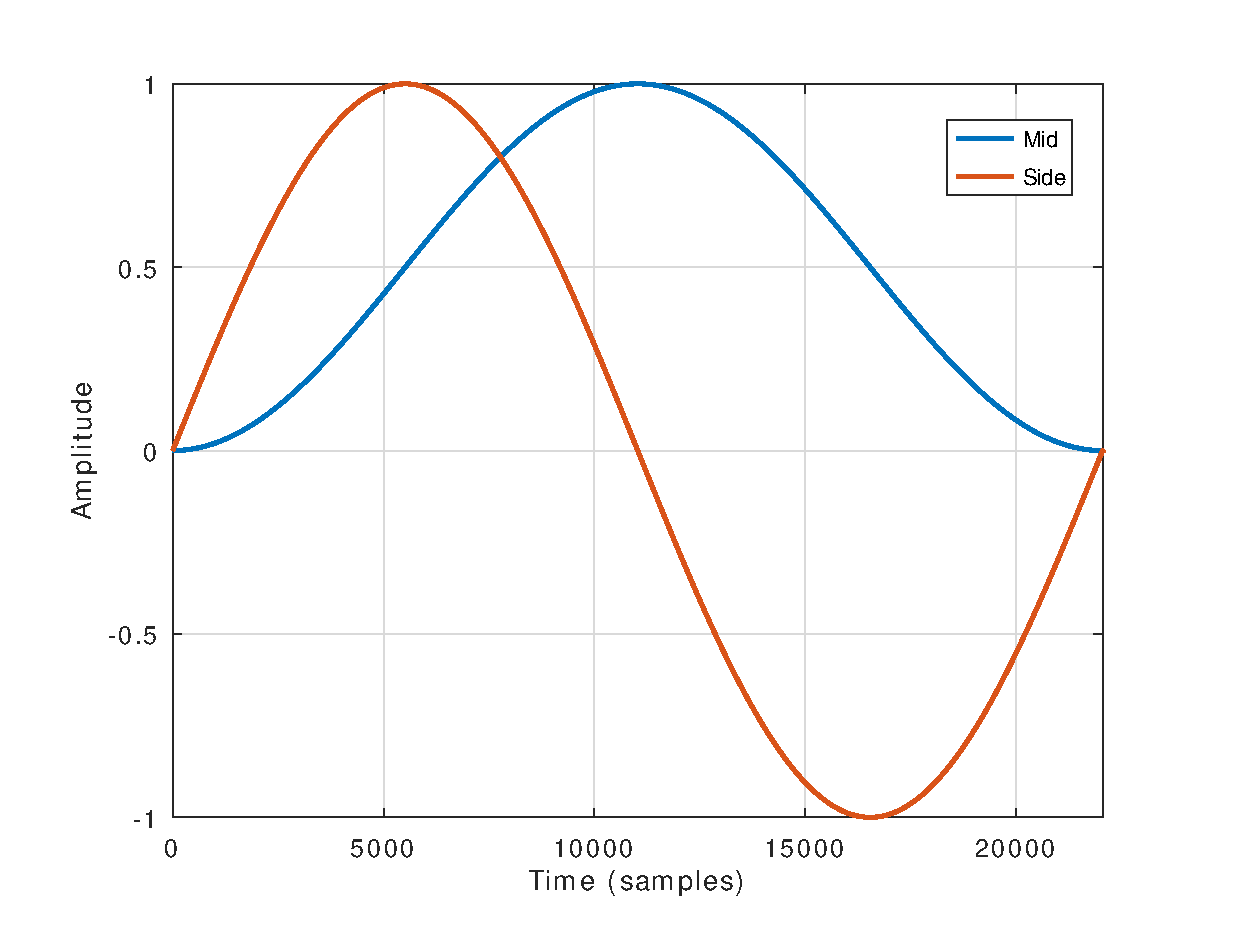
\includegraphics[width=1\columnwidth]{mspan}
\caption{Mid-Side panner, 360 degrees sweep from left to right. The Side (red) line shows the bipolarity of the signal related to angular information. The Mid (blue) line has only positive energy in relation to angular information. It is evident the zero meaning at both edges of -180 and 180 degrees, where cardioid and figure-8 are hear-less.}
\label{fig:mspan}
\end{figure}

%\section{Floats and equations}
%
%\subsection{Equations}
%Equations should be placed on separated lines and numbered. The number should be on the right side, in parentheses.
%\begin{equation}
%r=\sqrt[13]{3}
%\label{eq:BP}
%\end{equation}
%Always refer to equations like this: ``Equation (\ref{eq:BP}) is of particular interest because...''
%
%\subsection{Figures, Tables and Captions}
%\begin{table}[t]
% \begin{center}
% \begin{tabular}{|l|l|}
%  \hline
%  String value & Numeric value \\
%  \hline
%  Moin! SMC & 2020 \\
%  \hline
% \end{tabular}
%\end{center}
% \caption{Table captions should be placed below the table,  like this.}
% \label{tab:example}
%\end{table}
%
%All artwork must be centered, neat, clean and legible. Figures should be centered, neat, clean
%and completely legible. All lines should be thick and dark enough for purposes of reproduction. Artwork should not be hand-drawn. The proceedings will be distributed in electronic form only, therefore color figures are allowed. However, you may want to check that your figures are understandable even if they are printed in black-and-white.
%
%
%Numbers and captions of figures and tables always appear below the figure/table.
%Leave 1 line space between the figure or table and the caption.
%Figure and tables are numbered consecutively.
%Captions should be Times 10pt. Place tables/figures in the text as close to the reference as possible,
%and preferably at the top of the page.
%
%Always refer to tables and figures in the main text, for example: ``see Fig. \ref{fig:example} and \tabref{tab:example}''.
%Figures and tables may extend across both columns to a maximum width of 17.2cm.
%
%Vectorial figures are preferred, e.g., eps. When using \texttt{Matlab}, export using either (encapsulated) Postscript or PDF format. In order to optimize readability, the font size of text within a figure should be no smaller than
%that of footnotes (8~pt font-size). If you use bitmap figures, make sure that the resolution is high enough for print quality.

\begin{figure}[h]
\centering
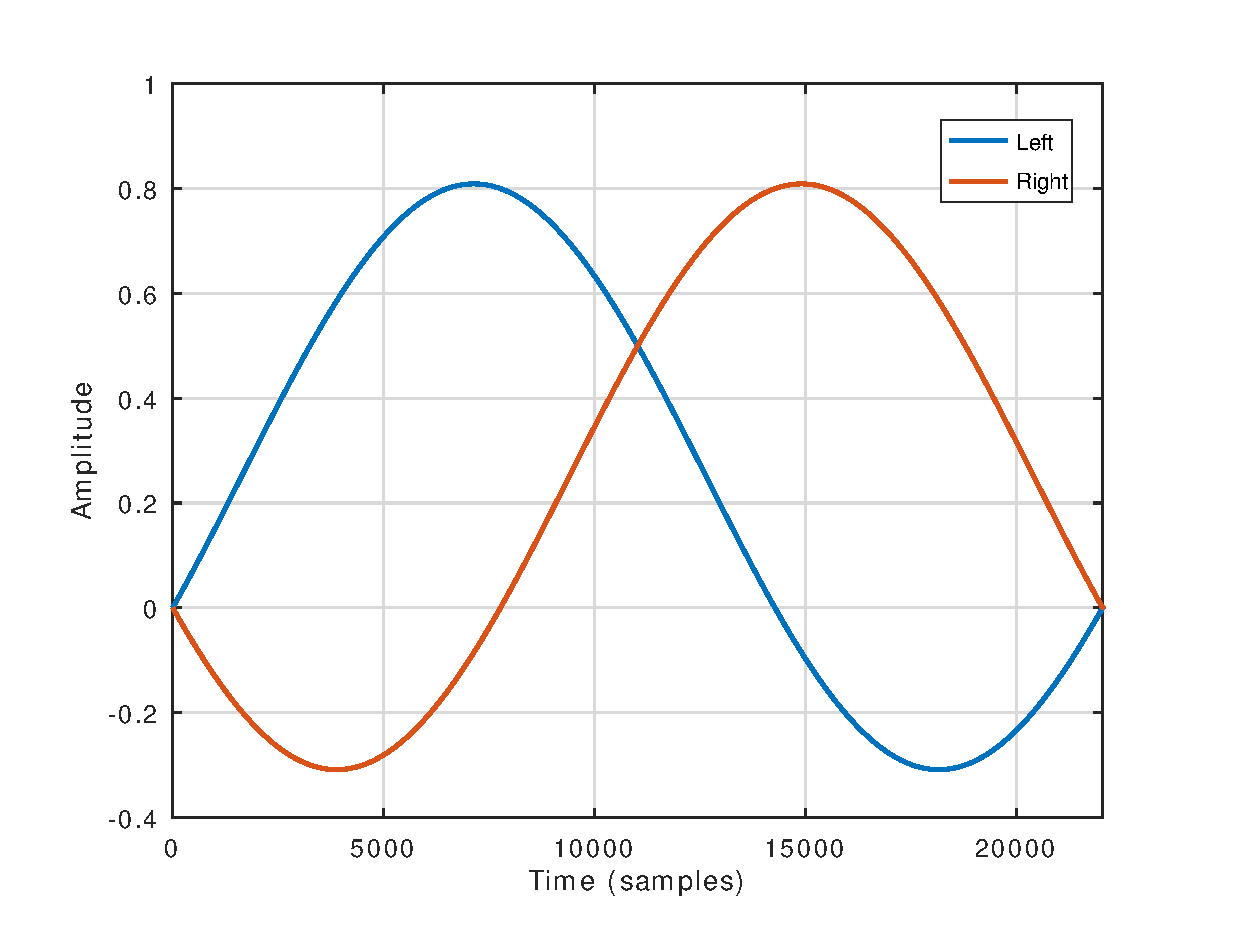
\includegraphics[width=1\columnwidth]{mspanlr}
\caption{Mid-Side panner to Left Right amplitude matrix. 360 degrees sweep from left to right. The top amplitude with cardioid polar pattern for the Mid channel is around 0.8. The 1 amplitude factor is reached when the Mid channel has an omnidirectional polar pattern.}
\label{fig:mspanlr}
\end{figure}

\vfill\null

\newpage
%%%%%%%%%%%%%%%%%%%%%%%%%%%%%%%%%%%%%%%%%%%%%%%%%%%%%%%%%%%%%%%%%% SECTION SEVEN
%%%%%%%%%%%%%%%%%%%%%%%%%%%%%%%%%%%%%%%%%%%%%%%%%%%%%%%%%%%%%%%%%%%%%%%%%%%%%%%%

\section{MS-PAN. Live usage}
\label{sec:mspanlive}

One of the most useful considerations of choosing panning techniques is usability in multiple circumstances. There are people who think quadratic panner is better than linear only because of its most recent introduction. They do not analyse the manual usage of one in place of the other. They do not analyse the mixer market and the role of panning in mass-culture music. Without analysing these practical issues, it is not really understandable why the worst panning technique ever is the most hardware implemented.  

We have explained the path to Mid-Side panning, starting from the roots. Now it is the moment to understand what possible usages are, what are the peculiarities of a Mid-Side panner instead of amplitude panners. 

The matrixed signal has its complexity as a disadvantage. To understand a signal as the significance of matrix combination requires a bit of tricky work more than straight signals. 

As musicians, even when plots and formulas are pretty clear, at the end of judgment, are the ears and the musical usability to determine the best, personal, choice. So, for us, for example, the phase modulation strength of the Mid-Side panner suggested, even before a practical test, better stability on live usages. It is pretty simple to demonstrate. A microphone is routed into a channel, with a mid-lateral pointed panner, and fed to the loudspeakers. With a quadratic panner, both left and right channels have the same phase. The feedback of signal inside the microphone has in-phase different energies. The feedback will increase quadratically. On the other hand, in the same feedback situation, with the same angular panning to the microphone signal, the Mid-Side panning will produce different phase and different energy for both loudspeakers. The differences, in air, will produce a more resistive feedback pattern. In other words, the Mid-Side panner act "naturally" as anti-Larsen.

\begin{figure}[h]
\centering
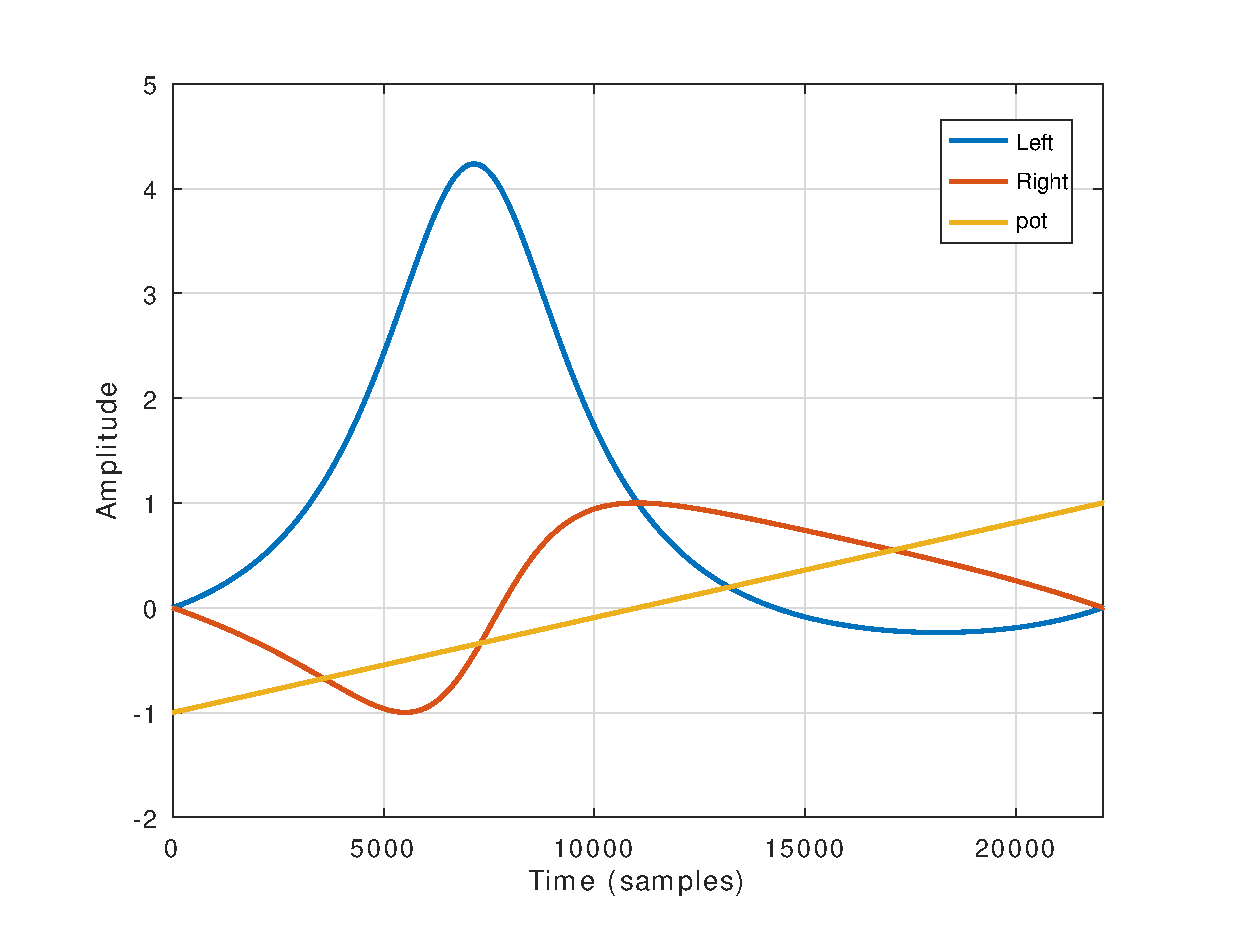
\includegraphics[width=1\columnwidth]{mspanlrfbpot}
\caption{Mid-Side to Left-Right panner. The plot describes the feedback response with a pan movement through the entire panorama, from -180 to 180 degrees (yellow line, normalized to -1 and 1). The energy multiplies up to four times for the left channel in infinite feedback (blue line). The top of feedback encreasing is at 45 degrees position in direction of the channel in feedback.}
\label{fig:mspanlrfb}
\end{figure}

\begin{figure}[h]
\centering
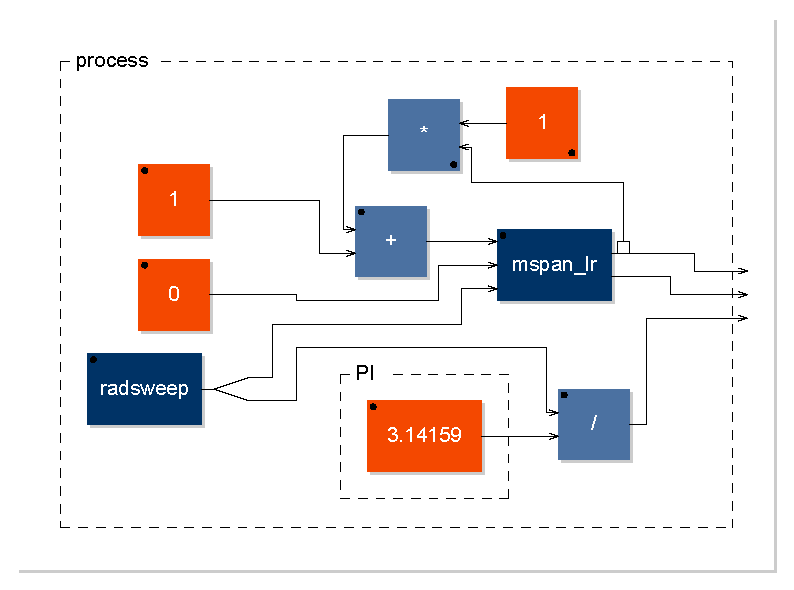
\includegraphics[width=1\columnwidth]{mspanlrfb_diagram}
\caption{Block diagram of the infinite feedback condition simulation on left channel. The sweep through all degrees is normalised to 1 for plotting purpose.}
\label{fig:mspan}
\end{figure}

To have an idea of live usability differences conditions, we plot the result of the same infinite loop for the Left Right quadratic panner. 

\begin{lstlisting}
lrpanq(x,p) = l,r
  with{
    l = sqrt(1-p)*x;
    r = sqrt(p)*x;
};
\end{lstlisting}

\begin{figure}[h]
\centering
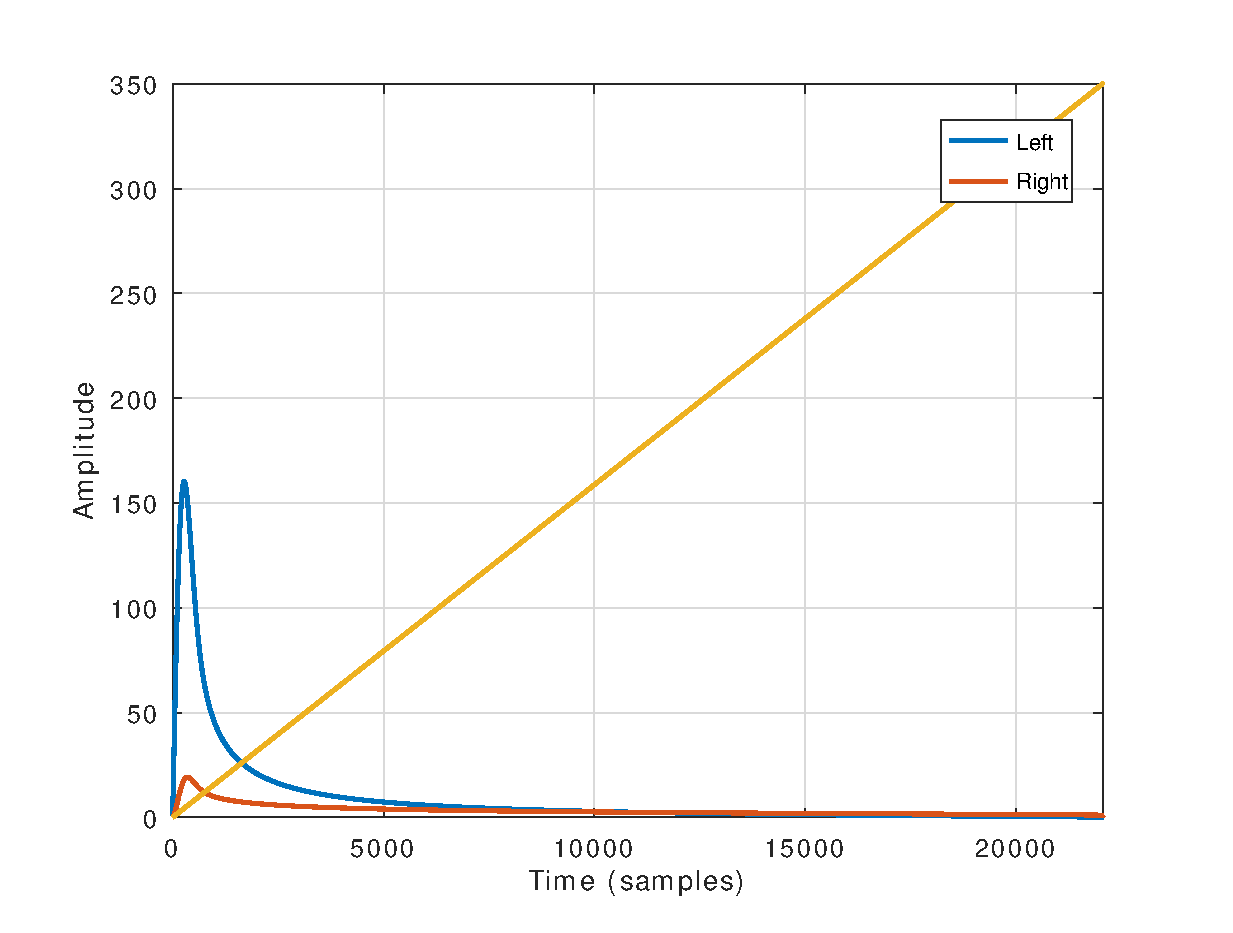
\includegraphics[width=1\columnwidth]{lrpanfbpot1}
\caption{Mid-Side panner to Left Right amplitude matrix. 360 degrees sweep from left to right.\label{fig:mspanlr}}
\end{figure}

\begin{figure}[t]
\centering
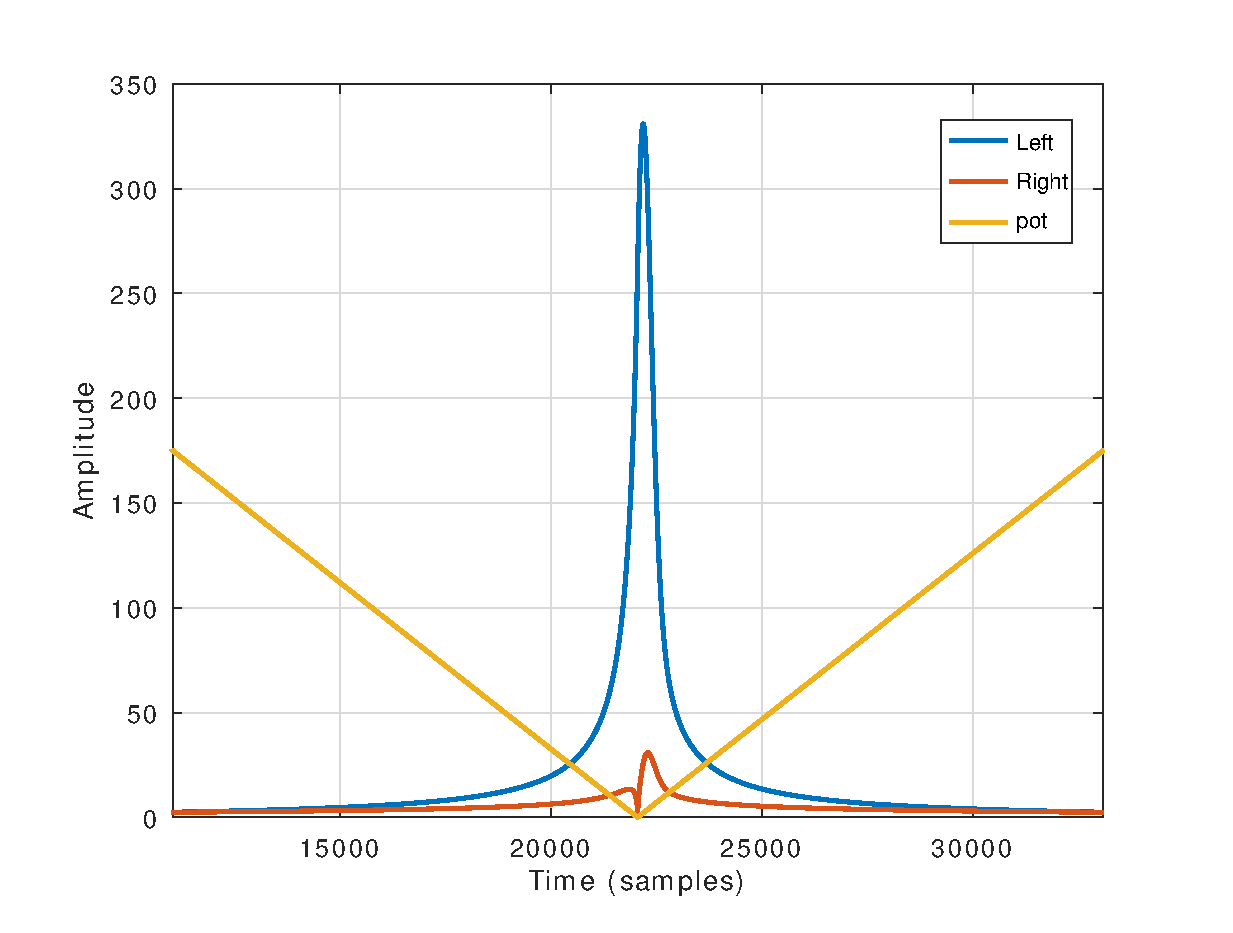
\includegraphics[width=1\columnwidth]{lrpanfbpot2}
\caption{Mid-Side panner to Left Right amplitude matrix. 360 degrees sweep from left to right.\label{fig:mspanlr}}
\end{figure}

\vfill\null

\newpage

%%%%%%%%%%%%%%%%%%%%%%%%%%%%%%%%%%%%%%%%%%%%%%%%%%%%%%%%%%%%%%%%%% SECTION SEVEN
%%%%%%%%%%%%%%%%%%%%%%%%%%%%%%%%%%%%%%%%%%%%%%%%%%%%%%%%%%%%%%%%%%%%%%%%%%%%%%%%
\section{CONCLUSIONS}
\label{sec:conc}

%\section{Citations}
%All bibliographical references should be listed at the end, inside a section named ``REFERENCES''. References must be numbered in order of appearance. You should avoid listing references that do not appear in the text.
%
%Reference numbers in the text should appear within square brackets, such as in~\cite{Someone:00} or~\cite{Someone:00,Someone:04,Someone:09}. The reference format is the standard IEEE one. We highly recommend you use BibTeX
%to generate the reference list.
%
%\section{Conclusions}
%Please, submit full-length papers. Submission is fully electronic and automated through the Conference Web Submission System. \underline{Do not} send papers directly by e-mail.
%
%
%\begin{acknowledgments}
%At the end of the Conclusions, acknowledgements to people, projects, funding agencies, etc. can be included after the second-level heading  ``Acknowledgments'' (with no numbering).
%\end{acknowledgments}

\vfill\null

\newpage

%%%%%%%%%%%%%%%%%%%%%%%%%%%%%%%%%%%%%%%%%%%%%%%%%%%%%%%%%%%%%%%%%%% BIBLIOGRAPHY
\bibliography{smc2020bib}

\end{document}
